Antes de conectar nuestro sistema con una base de datos de Firestore es necesario crear una aplicación en la consola de Google Firebase y seguir los siguientes pasos.
\vspace{0.8cm}

\begin{figure}[H]
  \centering
  
\includegraphics[width=1\textwidth]{firebase-01}
  \caption{Consola de Google Firebase.}
\end{figure}

\begin{enumerate}
  \item Crear un nuevo proyecto en la consola de Firebase.

  \begin{figure}[H]
    \centering
    
\includegraphics[width=1\textwidth]{firebase-02}
  \end{figure}

  \item En el apartado `Database', seleccionar `crear base de datos' .

  \begin{figure}[H]
    \centering
    
\includegraphics[width=1\textwidth]{firebase-03}
  \end{figure}

  \item En la ventana emergente, seleccionar reglas de seguridad y definir ubicación del servidor.

  \begin{figure}[H]
    \centering
    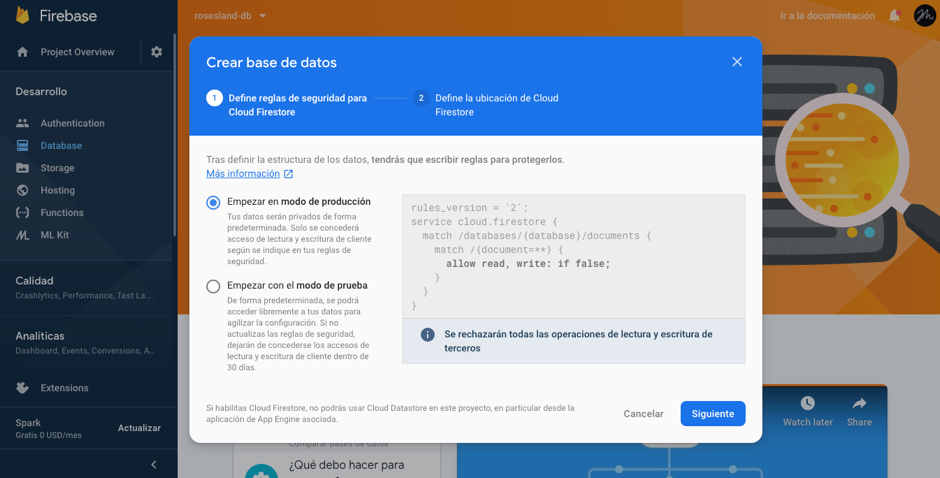
\includegraphics[width=1\textwidth]{firebase-04}
  \end{figure}

  \item El siguiente paso es generar las claves que permitan usar `firebase-admin' en el backend. En la configuración del proyecto debajo del apartado `cuentas de servicio', presionar el botón `Generar cuentas de servicio'. El contenido del archivo JSON generado se debe de agregar a las variables del entorno que correspondan.

  \begin{figure}[H]
    \centering
    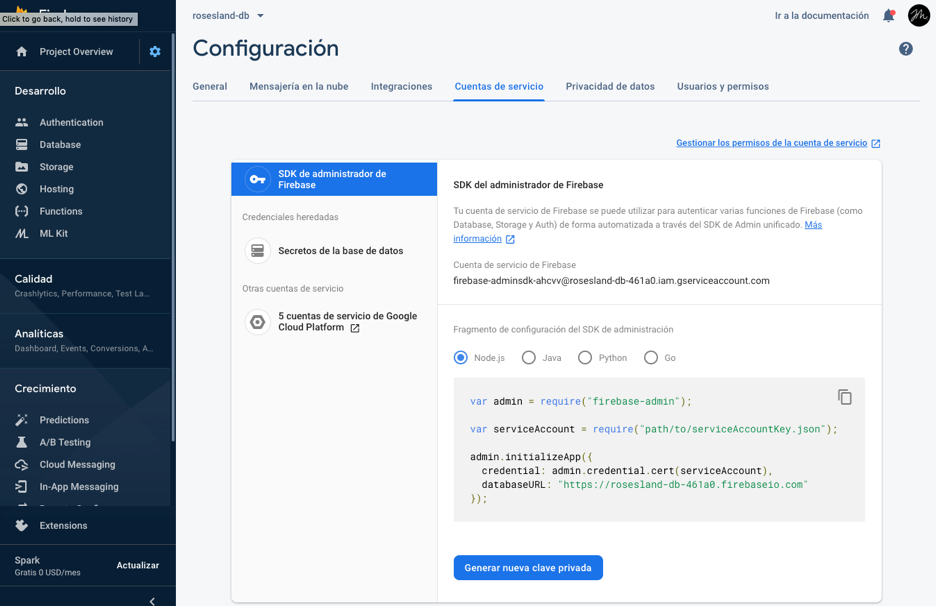
\includegraphics[width=1\textwidth]{firebase-05}
  \end{figure}

  \item Por ultimo en la sección `Authentication' se deben activar los servicios de autenticación necesarios, para este proyecto es necesario activar la validación por correo electrónico y contraseña.

  \begin{figure}[H]
    \centering
    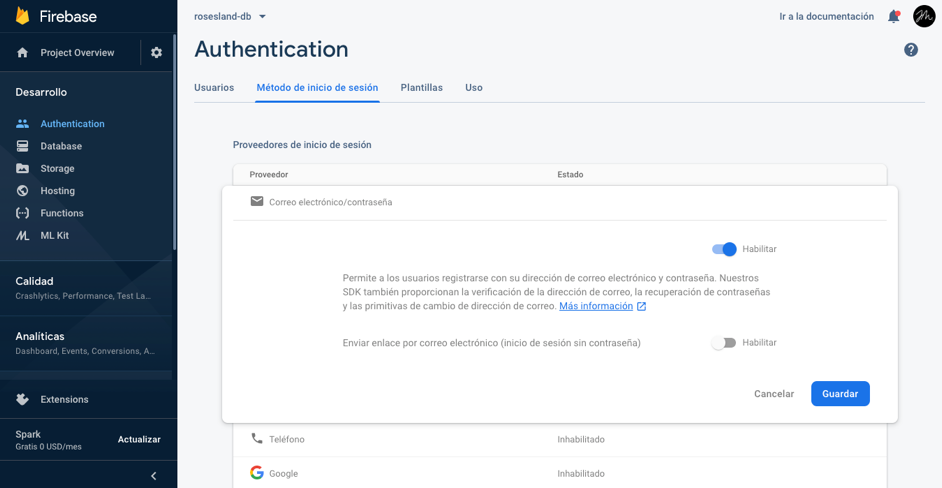
\includegraphics[width=1\textwidth]{firebase-06}
  \end{figure}
\end{enumerate}

\newpage
\subsubsection{Configuración de Firebase Firestore en Node.js}
Después de crear el objeto de configuración, es necesario inicializar Firebase en la aplicación de la siguiente manera:
\vspace{0.8cm}

\lstinputlisting[label={node-firebase}, style=ES6, caption=Fragmento de la configuración Firebase en el servidor]{code/firebase.js}

\subsubsection{Escrituras en lotes}
Para manipular documentos en un conjunto de operaciones, se pueden ejecutar varias operaciones de escritura como un lote único que incluya cualquier combinación de operaciones set(), update() o delete(). El lote de escrituras se completa de forma atómica y puede escribir en varios documentos. Los siguientes ejemplos muestran cómo crear y confirmar un lote de escrituras \cite{transactions}:
\vspace{0.8cm}

\lstinputlisting[label={firebase-function}, style=ES6, caption=Fragmento para guardar datos en Firestore]{code/firebase-function.js}


\subsection{Autenticación}
Casi todas las aplicaciones requieren algún sistema de autorización. En algunos casos, validar un nombre de usuario/contraseña establecido con nuestra tabla de Usuarios es suficiente, pero a menudo, necesitamos un modelo de permisos más detallado para permitir que ciertos usuarios accedan a ciertos recursos y los restrinjan de otros. Construir un sistema para soportar esto último no es trivial y puede llevar mucho tiempo. El API de autenticación basada en roles de Firebase, ayuda a poner todo en marcha rápidamente.

\subsubsection{Autenticación basada en roles}
En este modelo de autorización, se otorga acceso a roles, en lugar de usuarios específicos, y un usuario puede tener uno o más, según cómo diseñe su modelo de permiso. Los recursos, por otro lado, requieren ciertos roles para permitir que un usuario lo ejecute.
\vspace{0.8cm}

\begin{figure}[H]
  \centering
  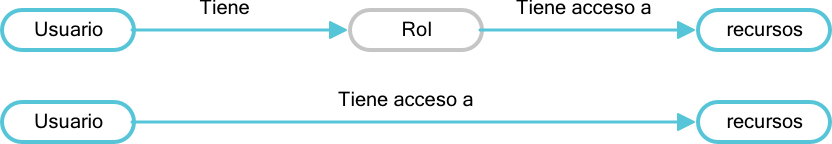
\includegraphics[width=1\textwidth]{firebase-auth}
  \caption{Autenticación basada en roles.}
\end{figure}

\subsubsection{Firebase Custom Claims}
Los roles de usuario son necesarios para identificar a los usuarios como administradores, gerentes o simplemente como clientes. Firebase Custom Claims permite establecer atributos de usuario simples directamente en el JWT del usuario (por ejemplo: \{ admin: true \}). Un JWT es un Json Web Token, es el objeto que contiene la información del usuario actual.
\vspace{0.8cm}

\lstinputlisting[label={firebase-auth}, style=ES6, caption=Fragmento para guardar crear y leer Firebase Custom Claims]{code/firebase-auth.js}